\documentclass[]{IEEEphot}

%\usepackage{cite}

\jvol{xx}
\jnum{xx}
\jmonth{June}
\pubyear{2009}

\newtheorem{theorem}{Theorem}
\newtheorem{lemma}{Lemma}

\begin{document}

\title{8 channel filter design  \\ With improvements to lower interbank }

\author{Tom Smy,\\   
Sanam Moslemi Tabriz}

\affil{Carleton 	University \\
Department of Electronics}  

%\doiinfo{DOI: 10.1109/JPHOT.2009.XXXXXXX\\
%1943-0655/\$25.00 \copyright 2009 IEEE}%

\maketitle

\markboth{IEEE Photonics Journal}{Volume }

%\begin{receivedinfo}%
%Manuscript received March 3, 2008; revised November 10, 2008. First published December 10, 2008. Current version published February 25, 2009. This research was sponsored by the National Science Foundation through the NSF ERC Center for Extreme Ultraviolet Science and Technology, NSF Award No. EEC-0310717. This paper was presented in part at the National Science Foundation.
%\end{receivedinfo}

\begin{abstract}
Step by step design of an eight channel filter using ring resonators and waveguide crossings. We also talk about solutions to minimize interbank crosstalk between channels.
\end{abstract}

\begin{IEEEkeywords}
Ring resonator, filter, inerband crosstalk, resonant splitting. 
\end{IEEEkeywords}

%\section{Introduction}

\section{Theory}
Here we studying the design and crosstalk in an n channel filter using ring resonators and waveguide crossings. There is two types of disruption happening in this circuits;
\begin{enumerate}
\item \textbf{Resonant splitting}

This effect happens because of poor filter design where the resonant peak and the FWHM of the individual channels interfere with each other, see 
Fig. ~\ref{resSpliting}. As shown in the Fig. ~\ref{resSpliting} channels 2, 5 and 6 are overlapping. To overcome resonant splitting, we need to properly design the structural parameters of the circuit based on the desired specification; bandwidth, channel's drop wavelength and $\dots$
\begin{figure}[h]
\vspace{-0.2cm}
\centering
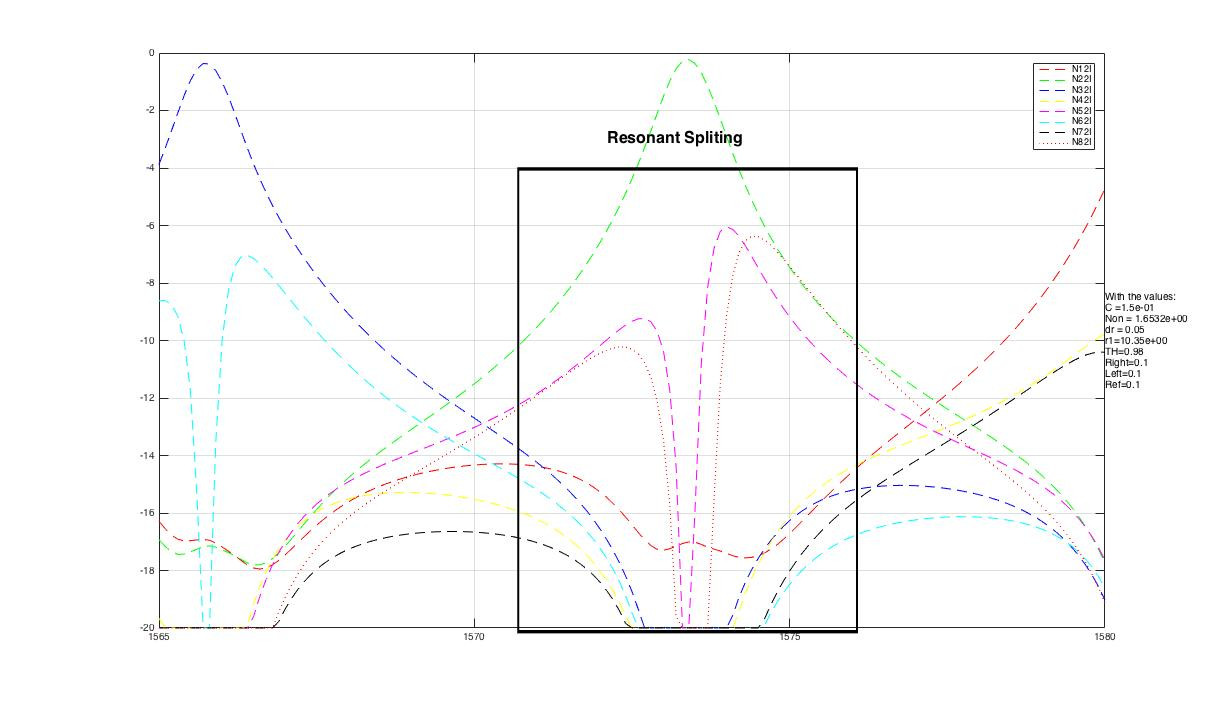
\includegraphics[width=30pc]{resSpliting}
\caption{Resonant splitting in the filter}
\label{resSpliting}
\end{figure}
\newpage
\item \textbf{Interband crosstalk}
Interband crosstalk happens between channels with different wavelength, where the power from unwanted adjacent channels interferes, shown in the Fig. ~\ref{crosstalkCH1NoDesignImv}. Interband crosstalk occurs out of spectral  band of a channel and that is why it won't effect resonant much. To overcome this issue we need to design High-Q filters with narrower bandwidth ~\cite{vahala}.
\begin{figure}[h]
\centering
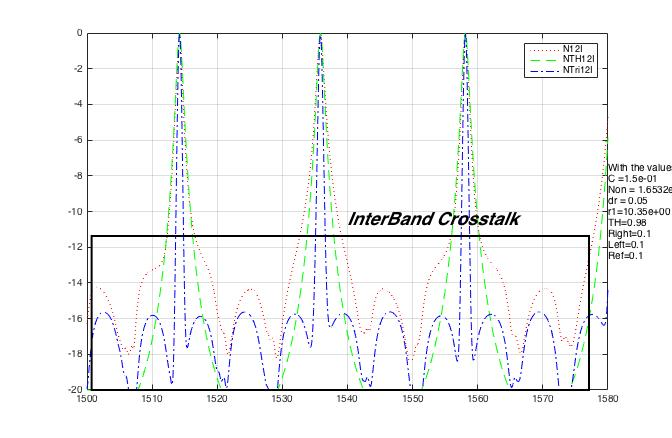
\includegraphics[width=30pc]{crosstalkCH1NoDesignImv}
\caption{Interbank crosstalk between channels}
\label{crosstalkCH1NoDesignImv}
\end{figure}
\end{enumerate}
\newpage
\section{Design details}
The purpose of this paper is to design an equally spaced n-channel filter with minimum interband disruption.
 \begin{equation}
m\lambda = n_{eff}L \qquad where\;m\;is\;an\;integer \quad and \quad L=2\pi R.
\label{lam} 
\end{equation}

\begin{equation}
FSR\;=\; \frac{\lambda^2}{n_{eff}L}
\label{FSR}
\end{equation}

\begin{equation}
\lambda_{1}^{(k)} = \lambda_{1}\;+\;(k-1).FSR \quad where\;k\;is\;an\;integer.
\end{equation}

Equation ~\ref{FSR} is only valid if we can ignore the dependency of index of reflection to wavelength. If this is not the case then we need to use $n_{g}$ which is the group index of reflection ~\cite{dgrabus}.

\begin{equation}
FSR\;=\; \frac{\lambda^2}{n_{g}L}
\label{FSRg}
\end{equation}
where
\begin{equation}
n_{g}\;=\;n_{eff}-\lambda_{0}\frac{\delta n_{eff}}{\delta\lambda}
\end{equation}
Channels are equally spaced by the value \begin{equation}
\Delta \lambda = \frac{FSR}{n} \quad where\;n\;is\;the\;number\;of\;channels
\end{equation}

\begin{equation}
\lambda_{n}=\lambda_{1} + (n-1)\Delta \lambda \quad where\;\lambda_{n}\;is\;the\;wavelength\;for\;the\;n_{th}\;channel.
\end{equation}

To overcome the resonant splitting, channel's linewidths must be designed in a way that channels don't overlap.
\begin{equation}
FWHM= \frac{(1-r^2a)\lambda^2}{\pi L n_{g}r\sqrt{a}} ~\cite{pub3105fsr}
\label{fwhm}
\end{equation}
\begin{equation}
r^2\;+\;\kappa ^2\;=\;1
\label{losslesscouplifng}
\end{equation}
where\begin{description}
\item[r] is the self coupling factor
\item[$\kappa$] is the cross coupling factor
\end{description}


%Equation ~\ref{fwhm} will set the maximum value of the cross-coupling coefficient ($\kappa$) to avoid resonant splitting. 

On the other hand if cross-coupling coefficient is too low, the bandwidth will be too narrow, so we need to optimize the cross-coupling coefficient. 

Bandwidth spec will define the minimum value of the cross-coupling coefficient. The cross-coupling coefficient has a close relation to the gap between the waveguide and the ring. To have a high $\kappa$, the gap must be very small, meaning the ring and waveguide must very close to each other and that has some fabrication difficulties.

\subsection{examples}
Design of an eight channel , equally spaced filter with the wavelength window of $1529-1551\;\; nm$. The minimum required bandwidth is $2\;THz$. 
For the simplicity assume $a=1$
Then for ring 1 (ch1) we have  $R_{1} = 10.30 \; \mu m$. ($n_{eff} =1.6532$ ~\cite{littlecbu1999}.)
Using ~\ref{lam}
\begin{equation}
\frac{\lambda_{n}}{\lambda_{1}^{(2)}}=\frac{R_{n}}{R_{1}}
\label{lamR}
\end{equation}
Note that in ~\ref{lamR} we chose $\lambda_{1}^{(2)}$ because of the window size and the direction we are moving in wavelength, see 
Table ~\ref{ChLamRSizes} for the channel's wavelength values and the associated ring sizes.

\begin{eqnarray*}
\Delta \lambda_{ch}\; =\; \frac{FSR}{n} \;=\;22 nm \\
\lambda_{n} \;= \;\lambda_{1}\;+\;(n-1)\Delta \lambda_{ch} \\
R_{n}\;=\;R_{1}\frac{\lambda_{n}}{\lambda_{1}^{(2)}}
 \end{eqnarray*}
\begin{table}[h]
\caption{Channel wavelength and Ring sizes}
\begin{center}
\begin{tabular}{|c|c|c|}
\hline
Ch. No. & Wavelength $nm$ & Ring size $\mu m$ \\
\hline
Ch1 & 1529 & 10.303 \\
\hline
Ch1 & 1531.75 & 10.172 \\
\hline
Ch1 & 1534.5 & 10.190\\
\hline
Ch1 & 1537.25 & 10.208 \\
\hline
Ch1 & 1540 & 10.226\\
\hline
Ch1 & 1542.75 & 10.244 \\
\hline
Ch1 & 1545.5 & 10.262 \\
\hline
Ch1 & 1548.25 & 10.28 \\
\hline
\end{tabular}
\end{center}
\label{ChLamRSizes}
\end{table}

To avoid resonant splitting for all channels (overlapping channels) and to meet the bandwidth spec,  we must fulfil the following constraints.
\begin{eqnarray}
\lambda_{k} +\frac{1}{2}FWHM_{k} < \lambda_{k+1} -\frac{1}{2}FWHM_{k+1} \qquad k\;=1,\; 2\; \dots \\
\Delta\lambda_{k}\;\equiv\; FWHM_{k} \qquad \qquad \qquad \qquad \nonumber
\label{minCoupCoef}
\end{eqnarray}
Equation \ref{minCoupCoef} will define the maximum value for $\kappa$ (cross-coupling coefficient).

\begin{eqnarray}
BW= c\frac{\Delta\lambda_{tat}}{\lambda^{2}} \qquad where\;c\;is\;the\;speed\;of\;light. \\
\Delta\lambda_{tat}\;=\;\Sigma_{1}^{n}\Delta\lambda_{i}  \qquad \qquad \qquad \qquad 
\label{BW}
\end{eqnarray}
Equation \ref{BW} will define the minimum value for $\kappa$ (cross-coupling coefficient).


\begin{figure}[h]
%\vspace{-0.2cm}
Fig. ~\ref{noResSpliYCrs} show the outputs of our filter. We see that resonant splitting is fixed and the crosstalk is lower. To improve the crosstalk more, we have used third order filters  by replacing each ring with 3 cascaded rings. Doing so, the size of the circuit is larger but crosstalk is much lower and the output is clean, see Fig. ~\ref{noResSpliNCrs}

\centering
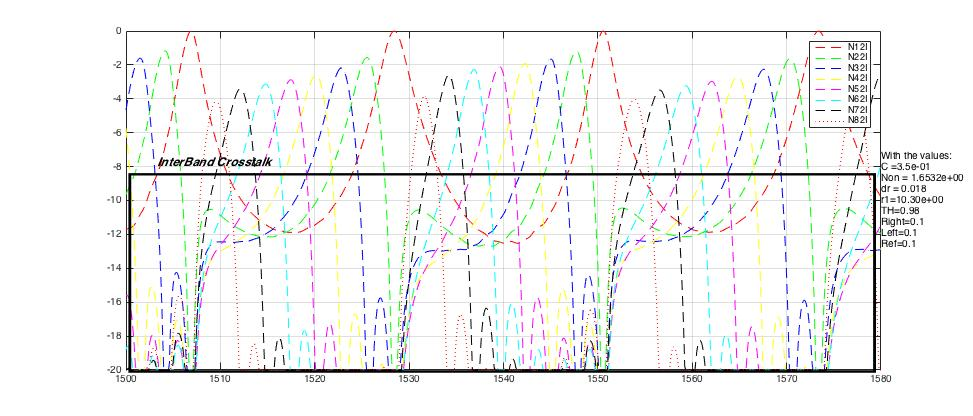
\includegraphics[width=30pc]{noResSpliYesCrstalk}
\caption{Fixed resonant splitting}
\label{noResSpliYCrs}
\end{figure}

\begin{figure}[h]
%\vspace{-0.2cm}
\centering
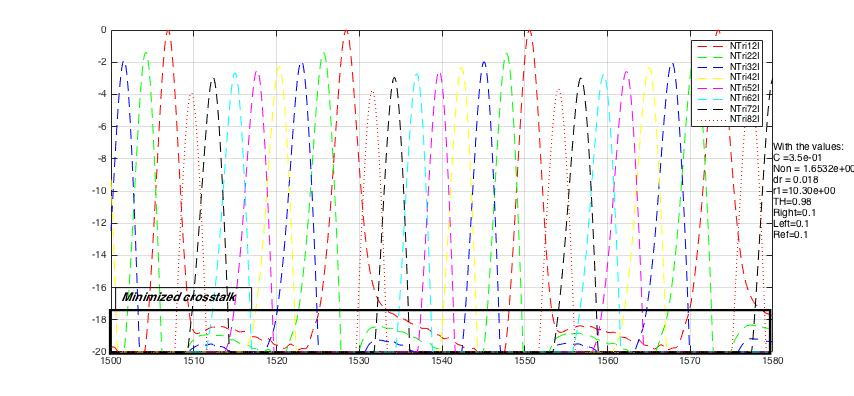
\includegraphics[width=30pc]{noResSpliNoCrstalk}
\caption{Improved crosstalk (interband}
\label{noResSpliNCrs}
\end{figure}




~\cite{oe1493872}

%\section{Experimental Details}
%
% The experimental set up is schematically illustrated in A compact $\alpha=46.9$ nm table top discharge-pumped capillary Ne-like Ar laser occupying only a 1 � 0.5 m2 footprint on an optical table was used for the recording of the hologram.    
%
%
%\subsection{Some Extra Details}
%
% Lasing was obtained in the 46.9 nm 3s 1P1 � 3p 1S0  transition of neon-like Ar by exciting Ar filled alumina capillaries 3.2 mm in diameter with a current pulse having an amplitude of 10\% to 90\% rise time of first half-cycle duration.  
%
%\subsubsection{Even more details}
%
% The pulse generator consists of a 4 stages Marx generator charged at voltages around 45 kV. The fast current pulse was produced by discharging a water dielectric cylindrical capacitor through a spark gap switch connected in series with the capillary load. The current pulse rapidly compresses the plasma column to achieve a dense and hot filamentary plasma channel where a population inversion is created by strong monopole electron impact excitation of the laser upper level and rapid radiative relaxation of the laser lower level. The water serves as a liquid dielectric for the capacitor and also cools the capillary.  
%
%
%\paragraph{A continuous} Flow of Ar is injected in the front of the capillary and an optimum Ar gas pressure of 490 mTorr is maintained in the capillary channel. The EUV laser and the vacuum chamber where the hologram was exposed, are connected via a vacuum manifold that provides differential pumping of the chamber that is maintained at ~ 10-5 Torr. The laser, operated with 18.4 cm long capillaries, produces 0.1J pulses at a repetition rate of 1 Hz 15. The high temporal and spatial  
%\begin{equation}
%x=\sum\limits_{1=0}^z 2^1Q
%\label{eq1}
%\end{equation}%
%coherence of the EUV table top laser permits the recording of large NA holograms for high resolution holographic imaging 18. The test object used in the holographic volume imaging experiment consisted of a tilted metallic surface covered with opaque spherical objects as can be seen in (\ref{eq1}). This test object was fabricated placing a 100 nm thick aluminum foil covering a hole 1.5 mm in diameter made in a 80 m thick mylar sheet. The hole was partially covered with a second mylar sheet 80 m thick, as schematically indicated in Fig.~\ref{fig_env2}.
%
%Humanoid robots have received much attention recently. Although they are able to walk without falling, their movements are not natural looking. In order for these robots to move more like humans, two technological obstacles need to be addressed: Firstly, there is a lack of flexibility in their body torsos. In all human activities, movements from the spine are involved. Yet, this important factor has been neglected by the majority of humanoid robotic researchers. One of the main reasons is that the added degrees of freedom (DOF) make it more costly and difficult to build a robot. Another key issue is that it is very difficult to program these types of robots so that they can maintain 
%balance. This numerical sectioning technique for holography is verified to produce a robust three dimension image of a test object. This numerical sectioning technique for holography is verified to produce a robust three dimension image of a test object.  This numerical sectioning technique for holography is verified to produce a robust three dimension image of a test object.   
%\setlength{\arraycolsep}{0.0em}
%\begin{eqnarray}
%Z&{}={}&x_1 + x_2 + x_3 + x_4 + x_5 + x_6 \nonumber\\
%&&+a + b\\
%&&+{}a + b\\
%&&{}+a + b\\
%&&{+}\:a + b
%\end{eqnarray}
%\setlength{\arraycolsep}{5pt}
%In order to address the above technological challenges, we need to develop flexible spine humanoid robots as experimental platforms. Recently, a few researchers have developed several spinal robots based on the anatomy of the human skeleton, Mizuuchi built a tendon-driven robot called {``}Kenta{"} \cite{Mizuuchi2002, Mizuuchi2003}. Although the robot has a spine, there has been no data to show that it can move in a flexible way. Also, the robot cannot stand up without external support because the upper body is too heavy \cite{Mizuuchi2003}. Mizuuchi later improved his prototype. However, it is also unable to 
%stand up without external support \cite{Mizuuchi2005,Nakanishi2007}.
% 
%At the German Space Agency (DLR), Hirzinger and his group developed a spine robot called {``}Justin{"}. The robot has a 3-DOF movable upper-torso, two arms and dexterous hands. Unlike the tendon-based robots developed by Mizuuchi and his colleagues, each controllable spinal joint of Justin is directly actuated by a DC Motor via a Harmonic Drive Gear. In order to prevent the robot from falling, the designers fixed the robot to a large platform \cite{Ott2006}. In November, 2007, researchers from Sugano Lab of Waseda University announced a new humanoid robot for household work and home care. The robot is called {``}Twendy-One{"}. It has a 4-DOF spine but it is fixed on a wheeled mobile platform. Thus, balancing is not an issue for this robot. It has a 4-DOF spine but it is fixed on a wheeled mobile platform. Thus, balancing is not an issue for this robot.
% 
%Inspired by the flexibility of belly dancers, Or conducted the first scientific study on belly dancing \cite{Or2006a}. He developed a database of belly dancing movements using computer animations. Later, Or recorded the movements of a professional belly dancer using a 12-camera VICON \cite{Mizuuchi2007} motion capture system. By analyzing the movements of the dancer, he developed a spinal mechanism which allows a full-body humanoid robot to exhibit all the human spine motions in 3D although with less degree of freedom \cite{Or2005a}. Moreover, the robot is able to stand up while performing dynamic torso motions without external support. In terms of controlling the mechanical spine, Or used a model of the lamprey central pattern generator. Experimental results showed that by using such neural networks, only three control parameters are needed to generate all human spinal motions. In order to conduct research on human-robot interactions, Or developed a new, full-body flexible spine humanoid robot  \cite{Or2007, Or2008}. Experimental results showed that it is possible for humans to perceive emotions expressed by a flexible spine humanoid robot. Later, Or developed the world{'s} first humanoid robot that can walk more naturally, like a human, with flexible spinal motions.
%
%
%The aluminum foil contours over the semicircular aperture to produce
%a variable height surface with the desirable characteristics for this
%test in Table~\ref{tab1}. The 100 nm aluminum foil has a transmission of approximately
%35\% at $\alpha=46.9$ nm considering the layer of native oxide 19 and
%effectively cuts the lower photon energy plasma emission from the Ar
%discharge in the laser source. 
%The sample was immersed in a solution of
%MIBK-methyl isobutyl ketone (4-Methyl-2- Pentanone) with IPA
%(isopropyl alcohol) 1:3 for 30 seconds, rinsed with IPA for 30
%seconds, and was finally dried using compressed
%nitrogen $x=\sum\limits_{1=0}^z 2^1Q$.
%
%%\begin{table}
%%\caption{This is an example of Table legend.}
%%\centering
%%\includegraphics{bozku.t1.eps}
%%\label{tab1}
%%\end{table}
%
%\begin{table}[!t]
%\centering
%\caption{Math Spacings Used By \LaTeX}
%\label{tab1}
%\begin{IEEEeqnarraybox}[\IEEEeqnarraystrutmode\IEEEeqnarraystrutsizeadd{2pt}{1pt}]{v/c/v/r/v/c/v/c/v/c/v}
%\IEEEeqnarrayrulerow\\
%& \mbox{{\bf Size}} && \mbox{{\bf Width}} && \mbox{{\bf Cmd.}} &&
%\mbox{{\bf Used for}} && \mbox{{\bf Example}} &\\
%\IEEEeqnarraydblrulerow\\
%\IEEEeqnarrayseprow[3pt]\\
%& \mbox{small} && \mbox{1/6 em} && \verb+\,+ && \mbox{symbols} && a b &\IEEEeqnarraystrutsize{0pt}{0pt}\\
%\IEEEeqnarrayseprow[3pt]\\
%\IEEEeqnarrayrulerow\\
%\IEEEeqnarrayseprow[3pt]\\
%& \mbox{medium} && \mbox{2/9 em} && \verb+\:+ && \mbox{binary operators} && a + b &\IEEEeqnarraystrutsize{0pt}{0pt}\\
%\IEEEeqnarrayseprow[3pt]\\
%\IEEEeqnarrayrulerow\\
%\IEEEeqnarrayseprow[3pt]\\
%& \mbox{large} && \mbox{5/18 em} && \verb+\;+ && \mbox{relational operators}&& a = b &\IEEEeqnarraystrutsize{0pt}{0pt}\\
%\IEEEeqnarrayseprow[3pt]\\
%\IEEEeqnarrayrulerow\\
%\IEEEeqnarrayseprow[3pt]\\
%& \mbox{negative small} && \mbox{${-}$1/6 em} && \verb+\!+ && \mbox{misc. uses} && ab &\IEEEeqnarraystrutsize{0pt}{0pt}\\
%\IEEEeqnarrayseprow[3pt]\\
%\IEEEeqnarrayrulerow
%\end{IEEEeqnarraybox}
%\end{table}
%
%\section{Results}
%
%We adjusted the\footnote{The aluminum foil contours over the semicircular aperture to produce a variable height surface with the desirable characteristics for this test. The 100 nm aluminum foil has a transmission of approximately 35\% at $\alpha=46.9$ nm considering the layer of native oxide 19 and effectively cuts the lower photon energy plasma emission from the Ar discharge in the laser source.} exposure so that the photoresist operated in a linear response regime. With exposure by the EUV laser, the holographic interference pattern generated by the reference and the object beams was recorded in the photoresist and converted to a surface modulation after the development.  Thus, the holograms were recorded as a relief pattern in the surface of a photoresist deposited on a Si wafer.
%\begin{itemize}
%\item Weight parameters for the simulated robot.
%\item Length of each body link.
%\item Specifications of body joints. Upper Torso means the spine. Due to symmetry, body parts from the right are not shown.
%\item Neuron parameters. $\Theta$ is the threshold, $\Gamma$ is the gain. $\tau_{D}$ and $\tau_{A}$ are respectively the time constant of the dendritic sums and that of the frequency adaptation. $\mu$ is the coefficient of frequency adaptation.
%\end{itemize}
%Holograms recorded in such a fashion can not be reconstructed in the conventional way with an optical reconstruction beam. In order to numerically reconstruct the holograms, the surface modulation was digitized with a Novascan atomic force microscope (AFM) operated in tapping mode. Holograms recorded in such a fashion can not be reconstructed in the conventional way with an optical reconstruction beam. In order to numerically reconstruct the holograms, the surface modulation was digitized with a Novascan atomic force microscope (AFM) operated in tapping mode. 
%\begin{enumerate}
%\item Screenshot of the Webots simulation environment.
%\item Schematic diagram of the simulated robot.
%\item Schematic of the model lamprey CPG. Connections with a dot ending represent inhibitory connections while those with an arrow ending represent excitatory connections.
%\item Sample output of a segmental oscillator (the 20th segment from the CPG). MNl and MNr respectively represents the output from the left and right motoneurons. Note the regularity of the neural pulses.
%\end{enumerate}
%
%\begin{table}[!t]
%\centering
%\caption{Possible $\Omega$ Functions}
%\label{tab2}
%\begin{IEEEeqnarraybox}[\IEEEeqnarraystrutmode\IEEEeqnarraystrutsizeadd{2pt}{1pt}]{v/c/v/c/v}
%\IEEEeqnarrayrulerow\\
%&\mbox{Range}&&\Omega(m)&\\
%\IEEEeqnarraydblrulerow\\
%\IEEEeqnarrayseprow[3pt]\\
%&x < 0&&\Omega(m)=\sum\limits_{i=0}^{m}K^{-i}&\IEEEeqnarraystrutsize{0pt}{0pt}\\
%\IEEEeqnarrayseprow[3pt]\\
%\IEEEeqnarrayrulerow\\
%\IEEEeqnarrayseprow[3pt]\\
%&x \ge 0&&\Omega(m)=\sqrt{m}\hfill&\IEEEeqnarraystrutsize{0pt}{0pt}\\
%\IEEEeqnarrayseprow[3pt]\\
%\IEEEeqnarrayrulerow
%\end{IEEEeqnarraybox}
%\end{table}
%
%\begin{table}[!t]
%\centering
%\caption{Network Delay as a Function of Load}
%\label{tab3}
%\begin{IEEEeqnarraybox}[\IEEEeqnarraystrutmode\IEEEeqnarraystrutsizeadd{2pt}{0pt}]{x/r/Vx/r/v/r/x}
%\IEEEeqnarraydblrulerowcut\\
%&&&&\IEEEeqnarraymulticol{3}{t}{Average Delay}&\\
%&\hfill\raisebox{-3pt}[0pt][0pt]{$\beta$}\hfill&&\IEEEeqnarraymulticol{5}{h}{}%
%\IEEEeqnarraystrutsize{0pt}{0pt}\\
%&&&&\hfill\lambda_{\mbox{min}}\hfill&&\hfill
%\lambda_{\mbox{max\vphantom{i}}}\hfill&\IEEEeqnarraystrutsizeadd{0pt}{2pt}\\
%\IEEEeqnarraydblrulerowcut\\
%&1&&& 0.057&& 0.172&\\
%&10&&& 0.124&& 0.536&\\
%&100&&& 0.830&& 0.905\rlap{\textsuperscript{*}}&\\
%\IEEEeqnarraydblrulerowcut\\
%&\IEEEeqnarraymulticol{7}{s}{\scriptsize\textsuperscript{*}limited usability}%
%\end{IEEEeqnarraybox}
%\end{table}
%
%Two holograms digitized in this manner are displayed in
%Fig.~\ref{fig_env2}.   The digital reconstruction of the hologram
%digitized by the AFM is based on a numerical Fresnel propagator in Table~\ref{tab2} and~\ref{tab3}. To obtain the amplitude and the phase distribution of the field in the image plane, the field emerging from the hologram illuminated by a plane wave is back propagated with the Fresnel-Kirchhoff integral. The integral was evaluated by the product of the spatial frequency representation of the hologram obtained through a two dimensional fast Fourier transformation and the quadratic phase free space Fresnel propagator in the spatial frequency domain.  
%
%\begin{theorem}[Einstein-Podolsky-Rosenberg]
%The back-propagation distance is determined by calculating the Fresnel zone plate (FZP) focal distance for the specific hologram geometry. For the specific geometry employed in this experiment, the FZP focal length is approximately the distance between the object and the recording medium. The digital images of the holograms processed with the Fresnel propagation code generated the reconstructed images shown in Fig.~\ref{fig_env2}.    
%\end{theorem}
%
%Holograms recorded in such a fashion can not be reconstructed in the conventional way with an optical reconstruction beam. In order to numerically reconstruct the holograms, the surface modulation was digitized with a Novascan atomic force microscope operated in tapping mode. 
%
%\begin{lemma}
%The back-propagation distance is determined by calculating the Fresnel zone plate (FZP) focal distance for the specific hologram geometry  For the specific geometry employed in this experiment, the FZP focal length is approximately the distance between the object and the recording medium. The digital images of the holograms processed with the Fresnel propagation code generated the reconstructed images shown in Fig.~\ref{fig_env2}.    
%\end{lemma}
%
%Holograms recorded in such a fashion can not be reconstructed in the conventional way with an optical reconstruction beam. In order to numerically reconstruct the holograms. 
%
%\begin{IEEEproof}%
%The back-propagation distance is determined by calculating the Fresnel zone plate (FZP) focal distance for the specific hologram geometry. For the specific geometry employed in this experiment, the FZP focal length is approximately the distance between the object and the recording medium. The digital images of the holograms processed with the Fresnel propagation code generated the reconstructed images shown in Fig.~\ref{fig_env2}.    
%\end{IEEEproof}
%
%\section{Conclusions}
% We have demonstrated that through detailed processing of the reconstructed holographic images, performed by changing the object-hologram distance in the reconstruction code, it is possible to discriminate depth in the object. Using a specially fabricated object composed of spherical markers 465 nm in diameter spread on a tilted transparent surface, the reconstruction and analysis of the hologram allowed to map the surface topography with a resolution close to 2 m, with such resolution depending on the particular NA of the exposure. 
%
%
%The lateral resolution of the image obtained by numerical reconstruction was assessed utilizing a wavelet image decomposition and image correlation. The best lateral resolution obtained with a high NA recording, 164 nm, represents an improvement of more than a factor two relative to previously published results.     
%
%\section*{Acknowledgements}
%The authors wish to thank the anonymous reviewers for their valuable suggestions.  
%
%%% \ackrule

\bibliographystyle{unsrt}
\bibliography{ring}

\end{document}
